\documentclass[border=2pt]{standalone}
\usepackage{tikz}
\usetikzlibrary{arrows.meta,chains}

\begin{document}
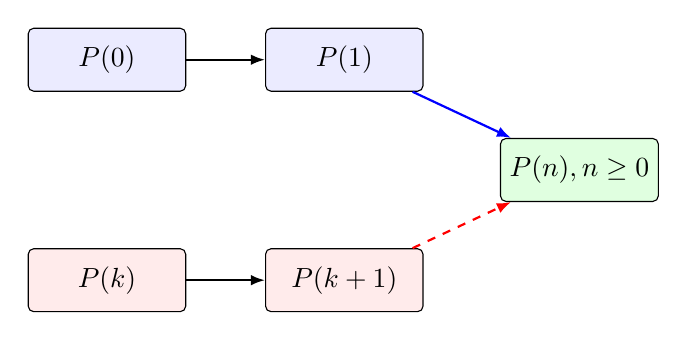
\begin{tikzpicture}[
  node distance=5mm and 10mm,
  start chain=base going right,
  start chain=step going right,
  start chain=proof going right,
  state/.style={draw,rounded corners=2pt,minimum width=20mm,minimum height=8mm,align=center},
  every on chain/.style={join},
  every join/.style={-{Latex[length=1.8mm]},thick}
]
  \node[state,on chain=base,fill=blue!8] (base-hypothesis) at (0,1.4) {$P(0)$};
  \node[state,on chain=base,fill=blue!8] (base-result) {$P(1)$};

  \node[state,on chain=step,fill=red!8] (step-hypothesis) at (0,-1.4) {$P(k)$};
  \node[state,on chain=step,fill=red!8] (step-result) {$P(k+1)$};

  \node[
    state,
    on chain=proof,
    fill=green!12,
    join=with base-end by {blue},
    join=with step-end by {red,dashed}
  ] (claim) at (6,0) {$P(n),n\geq0$};
\end{tikzpicture}
\end{document}
